\documentclass[12pt, letterpaper]{article}

% Packages
\usepackage[utf8]{inputenc}
\usepackage{geometry}
\usepackage{graphicx}
\usepackage{listings}
\usepackage{xcolor}
\usepackage{float}
\usepackage{enumitem}
\usepackage{array}
\usepackage{amsmath}

% Page Layout
\geometry{margin=1in}

% Header Information
\title{\textbf{Homework 3}}
\author{Yousef Alaa Awad}
\date{\today}

% Custom Formatting Commands
% Replaced \\ with \par to resolve Underfull \hbox warnings
\newcommand{\problem}[1]{\section*{Problem #1}}
\newcommand{\question}[1]{\noindent\textbf{Question: }#1\par\vspace{0.5em}}
\newcommand{\answer}{\noindent\textbf{Answer:}\par\vspace{1em}}

\begin{document}

\maketitle

\problem{1}
Suppose within your Web browser you click on a link to obtain a Web page. The IP address for the associated
URL is not cached in your local host, so a DNS lookup is necessary to obtain the IP address. Suppose that $n$
DNS servers are visited before your host receives the IP address from DNS; the successive visits incur an RTT
of $\text{RTT}_1, \dots, \text{RTT}_n$. Further suppose that the Web page associated with the link contains exactly
one object, consisting of a small amount of HTML text. Let $\text{RTT}_0$ denote the RTT between the local host
and the server containing the object.

\question{
  Assuming zero transmission time of the object, how much time elapses from when the client clicks on the link until
  the client receives the object?
}
\answer


\problem{2}
Referring to the above Problem 1, suppose the HTML file references eight very small objects on the same server.
Neglecting transmission times, how much time elapses with...

\begin{enumerate}[label=\alph*.]
	\item \textbf{Non-persistent HTTP with no parallel TCP connections} \newline
	      \answer

	\item \textbf{Non-persistent HTTP with the browser configured for 5 parallel connections} \newline
	      \answer

	\item \textbf{Persistent HTTP} \newline
	      \answer
\end{enumerate}


\problem{3}
Consider the Figure below, for which there is an institutional network connected to the Internet. Suppose that the 
average object size is $850,000$ bits and that the average request rate from the institution’s browsers to the origin
servers is 16 requests per second. Also suppose that the amount of time it takes from when the router on the Internet
side of the access link forwards an HTTP request until it receives the response is three seconds on average. Model the
total average response time as the sum of the average access delay (that is, the delay from Internet router to
institution router) and the average Internet delay. For the average access delay, use $\frac{\delta}{1-\delta\beta}$,
where $\delta$ is the average time required to send an object over the access link and $\beta$ is the arrival rate of
objects to the access link.

\begin{figure}[H]
	\centering
	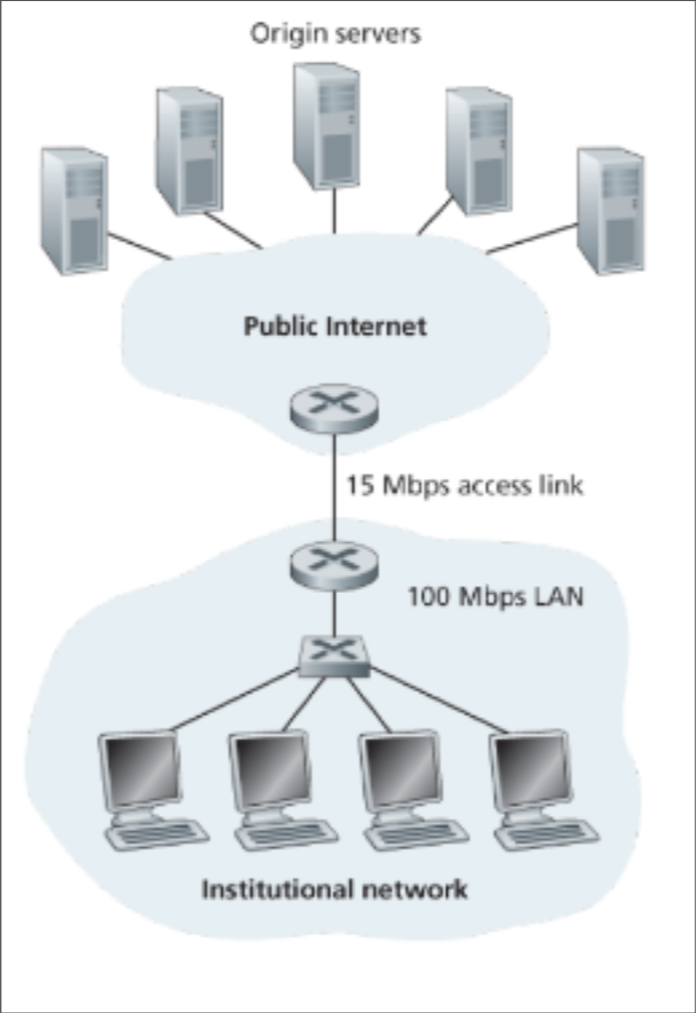
\includegraphics[width=0.3\textwidth]{q3figure.png}
\end{figure}

\begin{enumerate}[label=\alph*.]
	\item \textbf{Find the total average response time} \newline
	      \answer

	\item \textbf{Now suppose a cache is installed in the institutional LAN. Suppose the miss rate is 0.4. Find the
                total response time.
              } \newline
	      \answer
\end{enumerate}


\problem{4}
Consider distributing a file of $F = 15 \text{ Gbits}$ to $N$ peers. The server has an upload rate of $u_s = 30 
\text{ Mbps}$, and each peer has a download rate of $d_i = 2 \text{ Mbps}$ and an upload rate of $u$. For $N = 10$
and $1,000$ and $u = 300 \text{ Kbps}$ and $2 \text{ Mbps}$, prepare a chart giving the minimum distribution time
for each of the combinations of $N$ and $u$ for both client-server distribution and P2P distribution. \newline
\answer


\problem{5}
Consider distributing a file of $F$ bits to $N$ peers using a client-server architecture. Assume a fluid model where
the server can simultaneously transmit to multiple peers, transmitting to each peer at different rates, as long as the
combined rate does not exceed $u_s$.

\begin{enumerate}[label=\alph*.]
	\item \textbf{Suppose that $\frac{u_s}{N} \le d_{\min}$. Specify a distribution scheme that has a distribution time of $\frac{NF}{u_s}$.} \newline
	      \answer

	\item \textbf{Suppose that $\frac{u_s}{N} \ge d_{\min}$. Specify a distribution scheme that has a distribution time
                of $\frac{F}{d_{\min}}$.} \newline
	      \answer

	      % Moved equation to display math to resolve Overfull \hbox warning
	\item \textbf{Conclude that the minimum distribution time is in general given by:}
	      \[ \max\left(\frac{NF}{u_s}, \frac{F}{d_{\min}}\right) \]
	      \answer
\end{enumerate}


\problem{6}
Print out the header of an e-mail message you have recently received.

\begin{enumerate}[label=\alph*.]
	\item \textbf{How many \texttt{Received} header lines are there?} \newline
	      \answer

	\item \textbf{Why are there multiple \texttt{Received} header lines?} \newline
	      \answer
\end{enumerate}


\problem{7}
CDNs typically adopt one of two different server placement philosophies. Name and briefly describe them. \newline
\answer

\end{document}
